% Chapter Deployment
\chapter{Whirlpool Operations}
This chapter discusses server farm assembly for running whirlpool on a on-demand hardware resources offered by
AWS. It uses altitude analogy to illustrate important additions in infrastructure at various levels in
detail. The last section explains hardware configuration of resources used and their pricing details.

\section{Infrastructure from 10,000 feet}\label{infra10k}

Given a working knowledge of AWS and behavior of application that will run on top of its resources, it
becomes much easier to combine different tools to architect AWS solution. For this project, identical
copies of crawler application are deployed onto more than one machine. Special attention is paid to managing the state of the crawler. Combining understanding of theory discussed in section \ref{managestate}, intuition, and experience, the program maintains a global datastore(ContentDB) shared across all crawler processes. A running crawler process dumps downloaded data since the scope of the crawler for this thesis is confined to only data-collection. Also, the message broker RabbitMQ which forms the communication backbone is stateful(local) to a crawler process. So spinning each new crawler node will have its own RMQ bound to it. The internal metadata that crawler maintains which leverages a relational database and in-memory cache is also shared across crawler nodes to overcome scalability challenges and issues addressed in the theory of managing state in section \ref{managestate}. Lastly, the crawler program which forms the core business logic of
this thesis shouldn't be part of DMZ zone.
\\
\\
\noindent
Keeping above paragraph in mind, figure \ref{fig:infra10k} shows a AWS assembly containing four subnets
numbered 1-4 within a VPC. The Internet Gateway(IGW) is active and attached to this VPC. Public subnet 1 is explicitly associated with route table 1 which consist of route rule that directs traffic from subnet 1 to the outer public internet. The data transfer in crawling process is such that it will make connection
requests to the web sites and pull data into the amazon cloud, thus the inbound data transfer cost from
the internet into amazon cloud is free. Security-wise, the crawler nodes should never except incoming
connections from internet. These nodes are placed in private subnet 4. By default a private subnet within a AWS VPC is accessible to/from other subnets only within its VPC CIDR block and is denied any inbound/outbound
connections to the internet. As a best practice, subnet 4 is allowed only inbound connections. This is
done by associating subnet 4 with route table 2. A route in table 2 directs internet traffic to NAT instance deployed in public subnet 1 which further takes from Internet Gateway(IGW) attached to the VPC all the way into public internet.

\pagebreak

\begin{figure}[h!]
  \centering
  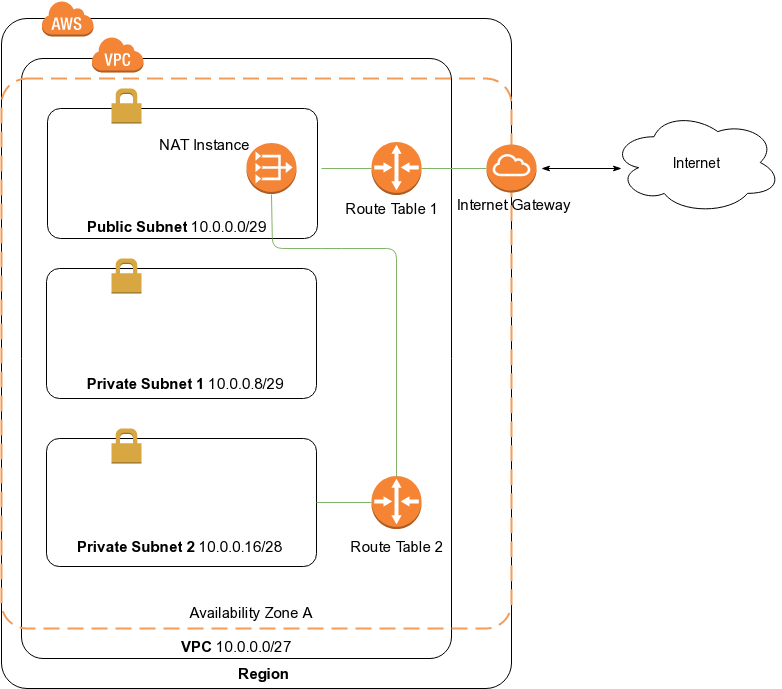
\includegraphics[width=18cm,height=12cm,keepaspectratio]{../media/crawler/ten-thousand-feet-aws.png}
  \caption{Whirlpool Infrastructure using VPC, AZ, and Subnet Sizing}
  \label{fig:infra10k}
\end{figure}

\noindent
The VPC in figure \ref{fig:infra10k} uses Classless Inter-Domain Routing(CIDR) block of \ipAddress{10.0.0.0/26} which
gives a range of \ipAddress{64} IPv4 addresses. This thesis uses a tool \cite{cidr} to calculate CIDR
blocks. AWS VPC reserves first four and last IPv4 addresses of each subnet created for internal usage and
therefore cannot be assigned to any instance of any resource. The primary CIDR block size of VPC is then
used to create 4 subnets each with a non-overlapping CIDR block size. The minimum
subnet size allowed is \ipAddress{28} and \ipAddress{16}.
\\
\\
CIDR block size is given by $2^{(32 - x)}$, substituting $x$ = 26 yields,
\begin{align*}
  2^{(32 - 26)} &= 64 && \text{IP addresses}
\end{align*}
\[
\text{4 subnets formation} = \underbrace{16}_\text{public subnet} + \overbrace{\underbrace{16}_\text{private db subnet 1} + \underbrace{16}_\text{private db subnet 2}}^\text{DB Subnet Group} + \underbrace{16}_\text{private crawler subnet} 
\\
\]
\[
\text{Actual IP addresses available} = \underbrace{11}_\text{public subnet} + \overbrace{\underbrace{11}_\text{private db subnet 1} + \underbrace{11}_\text{private db subnet 2}}^\text{DB Subnet Group} + \underbrace{11}_\text{private crawler subnet}
\]
\\
Public subnet IP range = \ipAddress{10.0.0.0/28} $\rightarrow$ (0 - 15)
\\                                                
Private db subnet 1 IP range = \ipAddress{10.0.0.16/28} $\rightarrow$ (16 - 31)
\\                                                
Private db subnet 2 IP range = \ipAddress{10.0.0.32/28} $\rightarrow$ (32 - 47)
\\
Private crawler subnet IP range = \ipAddress{10.0.0.48/28} $\rightarrow$ (48 - 64)